%!TEX root = ./Thesis.tex
\chapter[Projective interpolation for arbitrary parameterizations] % for the table of contents
{Projective interpolation for arbitrary parameterizations % normal title
\chaptermark{Projective interpolation} % title on the first page header of section
}
\chaptermark{Projective interpolation} % on other page headers of the sectioin

For discrete conformal maps \cite{Springborn2008} take advantage of a remarkable
property of discretely conformally equivalent meshes. Every triangle can be projectively 
mapped such that the circum circle is preserved. In fact this is a characterising property 
of discretely conformally equivalent meshes.

They arue that the circum circle preserving interpolation scheme gives visually better
results esecially for coarse meshes. We have observed that linear interpolation is a
particulary bad choice at cone singularities of the parameterization (Figure~\ref{fig:linear_projective_conformal}~left).

\begin{figure}
\centering
\resizebox{\textwidth}{!}{
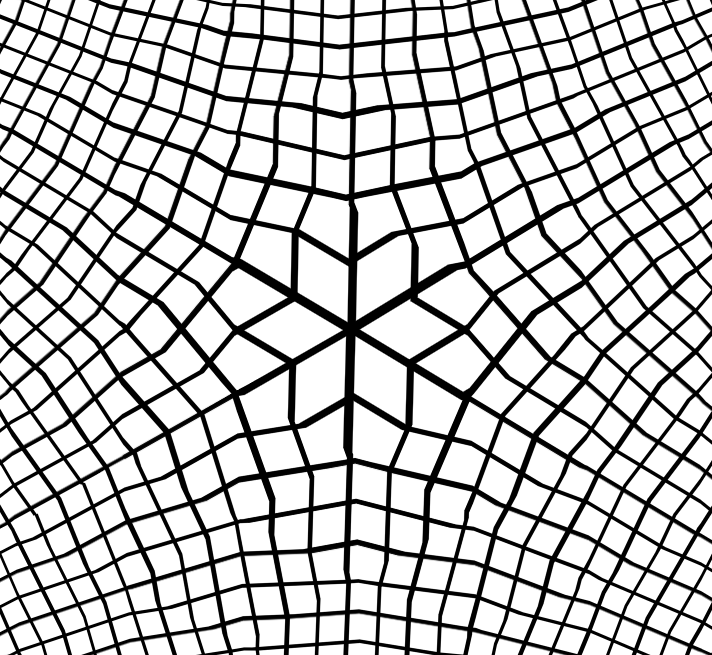
\includegraphics[width=0.33\textwidth]{image/projective/conformal_linear.png}
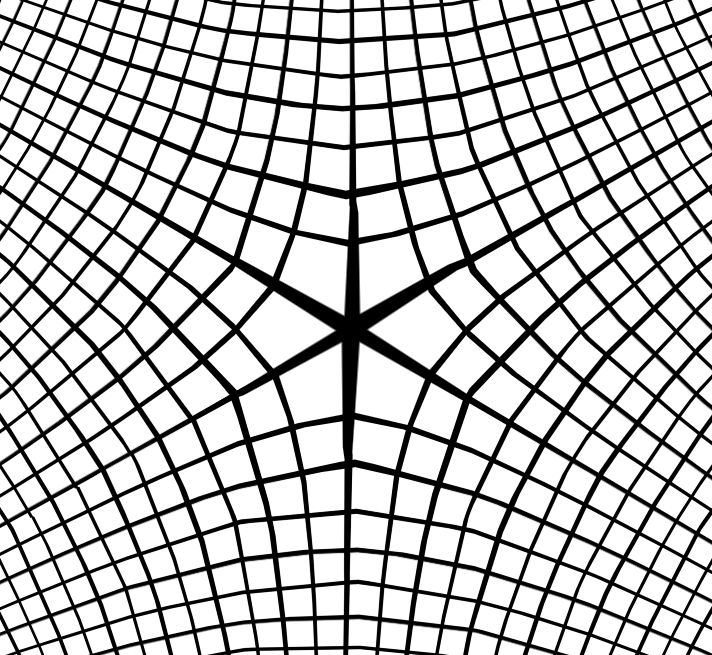
\includegraphics[width=0.33\textwidth]{image/projective/conformal_circum_circle.png}
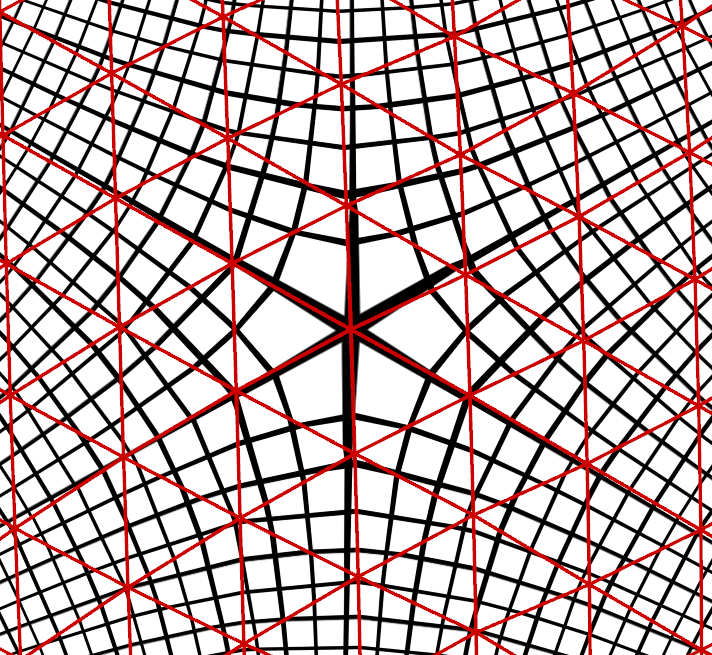
\includegraphics[width=0.33\textwidth]{image/projective/conformal_mesh.png}
}
\caption[Linear and projective interpolation]
{Linear (left) and circum circle preserving piece-wise projective (middle) interpolation 
at a cone-singularity of a coarse mesh (right) with vertices on a sphere. The parameterizatioin is discrete conformal.}
\label{fig:linear_projective_conformal} 
\end{figure}


Let $M=(V, E, F)$ be a triangulated surface consisting of vertices $i\in V$, edges $\it{ij}\in E$. 
Let $\lambda_{\it{ij}}$ be the logarithmic metric of the surface and $\tilde{\lambda}_{\it{ij}}$
be the logarithmic metric of the domain of a parameterization. In general $\lambda$ and 
$\tilde{\lambda}$ are not discretely conformally equivalent. The system of linear equations
\begin{equation}
	\lambda_{\it{ij}} + u_i + u_j = \tilde{\lambda}_{\it{ij}}
\end{equation}
has no solution $u\in \R^{|V|}$. 
We can however solve this system in a least squares fashion such that 
\[\sum_{\it{ij} \in E} \omega_{\it{ij}}(\lambda_{\it{ij}} + u_i + u_j - \tilde{\lambda}_{\it{ij}})^2 \]
is minimal. Where $\omega_{\it{ij}}$ is a weight per edge.

\begin{figure}
\centering
\resizebox{\textwidth}{!}{
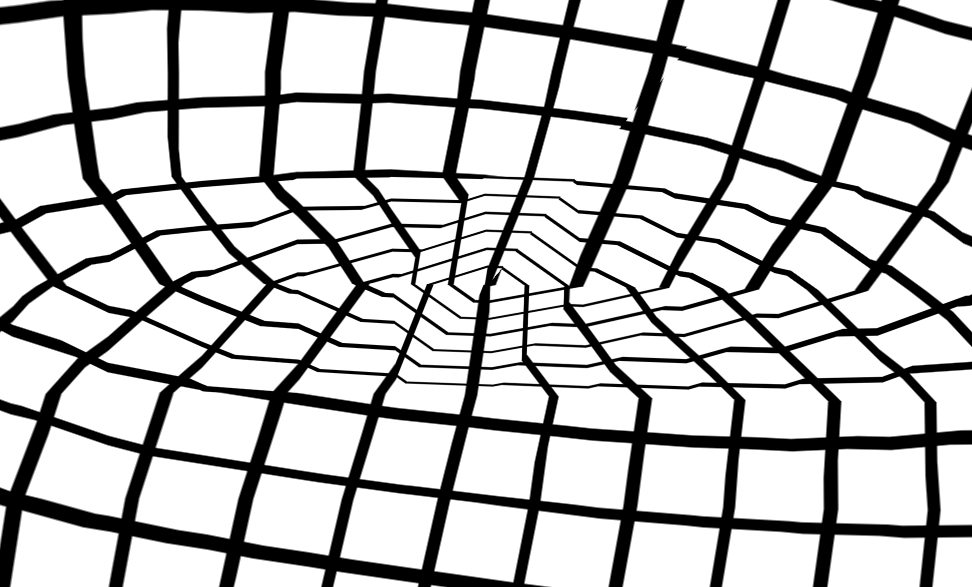
\includegraphics[width=0.33\textwidth]{image/projective/curvature_linear.png}
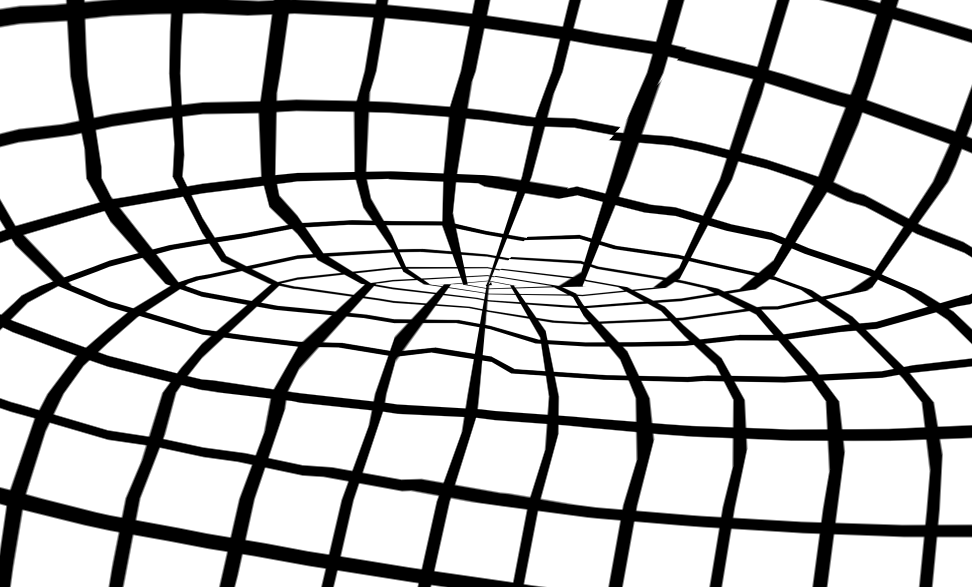
\includegraphics[width=0.33\textwidth]{image/projective/curvature_projective.png}
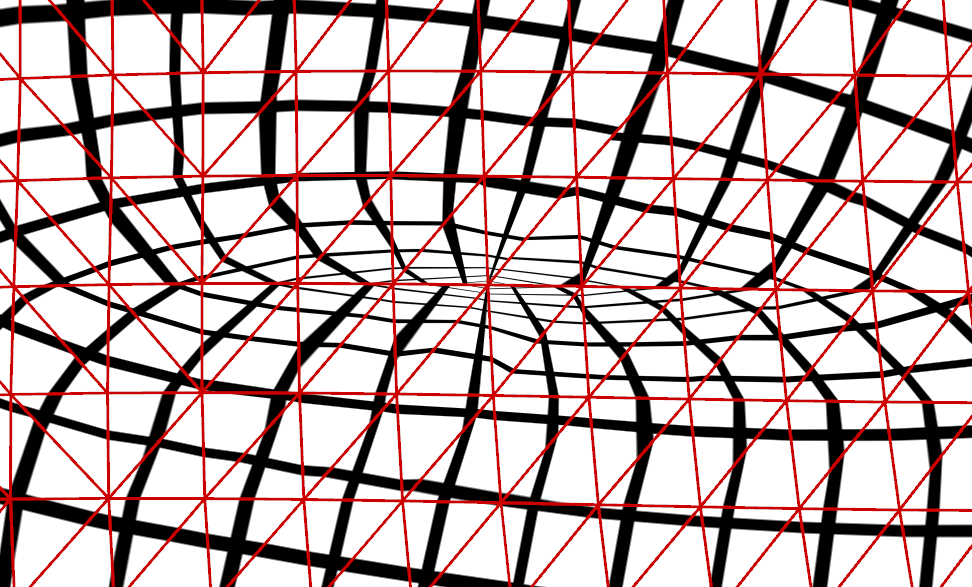
\includegraphics[width=0.33\textwidth]{image/projective/curvature_mesh.png}
}
\caption[Linear and projective interpolation at a cone-like singularity]
{Linear (left) and piece-wise projective (middle) interpolation 
at a cone-singularity of a coarse mesh (right). The parameterizatioin is not discrete conformal.}
\label{fig:linear_projective} 
\end{figure}


%%% Local Variables:
%%% TeX-master: "Thesis.tex"
%%% End: